\documentclass[twoside,11pt]{article}

\usepackage{aa228-jmlr2e}
\usepackage{lipsum}
\usepackage{listings}
\usepackage{geometry}
\geometry{margin=1in}

epackage[utf8]{inputenc}
\usepackage{textcomp}
\DeclareUnicodeCharacter{00B1}{\ifmmode\pm\else\textpm\fi}
\usepackage{listingsutf8}
\usepackage{mdframed}
\usepackage{xcolor}
%%
%% Julia syntax highlighting (c) Robert Moss
%%
\lstdefinelanguage{Julia}%
  {keywords=[2]{Tuple, flush, primes, Type, flush_cstdio, print, TypeConstructor, foldl, print_escaped, TypeError, foldr, print_joined, TypeName, print_shortest, TypeVar, frexp, print_unescaped, UTF16String, full, print_with_color, UTF32String, fullname, println, UTF8String, process_exited, UdpSocket, functionloc, process_running, Uint, functionlocs, procs, Uint128, gamma, prod, Uint16, gc, prod!, Uint32, gc_disable, produce, Uint64, gc_enable, promote, Uint8, gcd, promote_rule, UndefRefError, gcdx, promote_shape, UndefVarError, gensym, promote_type, UniformScaling, get, push!, Union, get!, pushdisplay, UnionType, get_bigfloat_precision, put, UnitRange, get_bigfloat_rounding, put!, Unsigned, get_rounding, pwd, VERSION, getaddrinfo, qr, Vararg, getfield, qrfact, VecOrMat, gethostname, qrfact!, Vector, getindex, quadgk, VersionNumber, getipaddr, quantile, Void, getkey, quantile!, WORD_SIZE, getpid, quit, WString, givens, WeakKeyDict, global, rad2deg, WeakRef, golden, radians2degrees, WindowsRawSocket, gperm, rand, Woodbury, gradient, rand!, Zip, hankelh1, randbool, hankelh1x, randbool!, hankelh2, randcycle, abs, hankelh2x, randn, abs2, hash, randn!, abspath, haskey, randperm, hcat, randstring, accept, help, randsubseq, @MIME, acos, hessfact, randsubseq!, @MIME_str, acosd, hessfact!, range, @__FILE__, acosh, hex, rank, @allocated, acot, hex2bytes, rationalize, @assert, acotd, hex2num, read, @async, acoth, hist, read!, @b_str, acsc, hist2d, readall, @bigint_str, acscd, histrange, readandwrite, @boundscheck, acsch, homedir, readavailable, @cmd, addprocs, htol, readbytes, @code_llvm, airy, hton, readbytes!, @code_lowered, airyai, hvcat, readchomp, @code_native, airyaiprime, hypot, readcsv, @code_typed, airybi, iceil, readdir, @deprecate, airybiprime, idct, readdlm, @edit, airyprime, idct!, readline, @elapsed, airyx, identity, readlines, @eval, all, readsfrom, @evalpoly, all!, ifelse, readuntil, @everywhere, angle, ifft, real, @fetch, ans, ifft!, realmax, @fetchfrom, any, ifftshift, realmin, @gensym, any!, ifloor, realpath, @goto, append!, ignorestatus, recv, @inbounds, applicable, im, redirect_stderr, @int128_str, apply, imag, redirect_stdin, @ip_str, apropos, redirect_stdout, @label, ascii, redisplay, @less, asec, reduce, @linux, asecd, in, reducedim, @linux_only, asech, include, reenable_sigint, @mstr, asin, include_string, reim, @non_windowsxp_only, asind, ind2chr, reinterpret, @osx, asinh, ind2sub, reload, @osx_only, assert, indexin, rem, @parallel, atan, indexpids, rem1, @printf, atan2, indmax, remotecall, @profile, atand, indmin, remotecall_fetch, @r_mstr, atanh, inf, remotecall_wait, @r_str, atexit, info, repeat, @schedule, backtrace, infs, replace, @show, baremodule, insert!, repmat, @simd, base, int, repr, @spawn, base64, int128, reprmime, @spawnat, basename, int16, require, @sprintf, int32, reset, @sync, beginswith, int64, reshape, @task, besselh, int8, resize!, @thunk, besseli, integer, rethrow, @time, besselix, interrupt, @timed, besselj, intersect, reverse, @uint128_str, besselj0, intersect!, reverse!, @unexpected, besselj1, inv, rfft, @unix, besseljx, invdigamma, rm, @unix_only, besselk, invmod, rmdir, @v_str, besselkx, invoke, rmprocs, @vectorize_1arg, bessely, invperm, rol, @vectorize_2arg, bessely0, ipermute!, ror, @which, bessely1, ipermutedims, rot180, @windows, besselyx, irfft, rotl90, @windows_only, beta, iround, rotr90, @windowsxp_only, bfft, is, round, ANY, bfft!, is_assigned_char, rpad, ARGS, big, is_valid_ascii, rref, ASCIIString, bin, is_valid_char, rsearch, A_ldiv_B!, bind, is_valid_utf16, rsearchindex, A_ldiv_Bc, binomial, is_valid_utf8, rsplit, A_ldiv_Bt, bitbroadcast, isa, rstrip, A_mul_B!, bitmix, isabspath, run, A_mul_Bc, bitpack, isalnum, scale, A_mul_Bc!, bits, isalpha, scale!, A_mul_Bt, bitstype, isapprox, schedule, A_mul_Bt!, bitunpack, isascii, schur, A_rdiv_Bc, bkfact, isbits, schurfact, A_rdiv_Bt, bkfact!, isblank, schurfact!, AbstractArray, blas_set_num_threads, isblockdev, sdata, AbstractMatrix, blkdiag, ischardev, search, AbstractRNG, bool, iscntrl, searchindex, AbstractSparseArray, break, isconst, searchsorted, AbstractSparseMatrix, brfft, isdefined, searchsortedfirst, AbstractSparseVector, broadcast, isdigit, searchsortedlast, AbstractVecOrMat, broadcast!, isdir, sec, AbstractVector, broadcast!_function, isdirpath, secd, Ac_ldiv_B, broadcast_function, iseltype, sech, Ac_ldiv_Bc, broadcast_getindex, isempty, seek, Ac_mul_B, broadcast_setindex!, isequal, seekend, Ac_mul_B!, bswap, iseven, seekstart, Ac_mul_Bc, bytes2hex, isexecutable, select, Ac_mul_Bc!, bytestring, isfifo, select!, Ac_rdiv_B, c_calloc, isfile, send, Ac_rdiv_Bc, c_free, isfinite, serialize, Any, c_malloc, isgeneric, set_bigfloat_precision, ArgumentError, c_realloc, isgraph, set_bigfloat_rounding, Array, cartesianmap, ishermitian, set_rounding, Associative, cat, isimmutable, setdiff, At_ldiv_B, catalan, isinf, setdiff!, At_ldiv_Bt, isinteger, setenv, At_mul_B, catch_backtrace, isinteractive, setfield, At_mul_B!, cbrt, isleaftype, setfield!, At_mul_Bt, ccall, isless, setindex!, At_mul_Bt!, cd, islink, shift!, At_rdiv_B, ceil, islower, show, At_rdiv_Bt, cell, ismarked, showall, BLAS, cfunction, ismatch, showcompact, Base, cglobal, isnan, showerror, Base64Pipe, char, isodd, shuffle, Bidiagonal, charwidth, isopen, shuffle!, BigFloat, checkbounds, ispath, sign, BigInt, chmod, isperm, signbit, BitArray, chol, isposdef, signed, BitMatrix, cholfact, isposdef!, signif, BitVector, cholfact!, ispow2, significand, Bool, chomp, isprime, similar, BoundsError, chop, isprint, sin, Box, chr2ind, ispunct, sinc, ByteString, circshift, isqrt, sind, CFILE, cis, isreadable, sinh, CPU_CORES, clamp, isreadonly, sinpi, C_NULL, clear_malloc_data, isready, size, Cchar, clipboard, isreal, sizehint, Cdouble, close, issetgid, sizeof, Cfloat, cmp, issetuid, skip, Char, code_llvm, issocket, skipchars, CharString, code_lowered, issorted, sleep, Cint, code_native, isspace, slice, Clong, code_typed, issparse, slicedim, Clonglong, collect, issticky, sort, ClusterManager, colon, issubnormal, sort!, Cmd, combinations, issubset, sortcols, Coff_t, complement, issubtype, sortperm, Collections, complement!, issym, sortrows, Colon, complex, istaskdone, sparse, Complex, complex128, istext, sparsevec, Complex128, complex32, istril, spawn, Complex32, complex64, istriu, spdiagm, Complex64, cond, isupper, speye, Condition, condskeel, isvalid, splice!, Core, conj, iswritable, split, Cptrdiff_t, conj!, isxdigit, splitdir, Cshort, connect, itrunc, splitdrive, Csize_t, join, splitext, Cssize_t, consume, joinpath, spones, Cuchar, contains, keys, sprand, Cuint, kill, sprandbool, Culong, conv, kron, sprandn, Culonglong, conv2, last, sprint, Cushort, convert, lbeta, spzeros, Cwchar_t, copy, lcfirst, sqrt, DArray, copy!, lcm, sqrtm, DL_LOAD_PATH, copysign, ldexp, squeeze, DataType, cor, ldltfact, srand, DenseArray, cos, ldltfact!, start, DenseMatrix, cosc, leading_ones, start_reading, DenseVecOrMat, cosd, leading_zeros, start_timer, DenseVector, cosh, length, start_watching, DevNull, cospi, less, stat, Diagonal, cot, let, std, Dict, cotd, lexcmp, stdm, DimensionMismatch, coth, lexless, step, Dims, count, lfact, stop_reading, DirectIndexString, count_ones, lgamma, stop_timer, Display, count_zeros, linrange, strerror, DivideError, countlines, linreg, strftime, DomainError, countnz, linspace, stride, ENDIAN_BOM, cov, listen, strides, ENV, cp, listenany, string, EOFError, cross, local, stringmime, EachLine, csc, localindexes, strip, Enumerate, cscd, localpart, strptime, ErrorException, csch, log, strwidth, Exception, ctime, log10, sub, Expr, ctranspose, log1p, sub2ind, FFTW, cummax, log2, subtypes, Factorization, cummin, logdet, success, FileMonitor, cumprod, logspace, sum, FileOffset, cumprod!, lowercase, sum!, Filter, cumsum, lpad, sum_kbn, Float16, cumsum!, lstat, sumabs, Float32, cumsum_kbn, lstrip, sumabs!, Float64, current_module, ltoh, sumabs2, FloatRange, current_task, lu, sumabs2!, FloatingPoint, dawson, lufact, summary, Function, dct, lufact!, super, GetfieldNode, dct!, lyap, svd, GotoNode, dec, svdfact, Graphics, deconv, macroexpand, svdfact!, Hermitian, deepcopy, map, svdvals, I, deg2rad, map!, svdvals!, IO, degrees2radians, mapreduce, sylvester, IOBuffer, delete!, mapslices, symbol, IOStream, deleteat!, mark, symdiff, IPv4, den, match, symdiff!, IPv6, dense, matchall, symlink, InexactError, deserialize, max, symperm, Inf, det, maxabs, systemerror, Inf16, detach, maxabs!, take, Inf32, dfill, maximum, take!, InsertionSort, diag, maximum!, takebuf_array, Int, diagind, maxintfloat, takebuf_string, Int128, diagm, mean, tan, Int16, diff, mean!, tand, Int32, digamma, median, tanh, Int64, digits, median!, task_local_storage, Int8, dirname, merge, tempdir, IntSet, disable_sigint, merge!, tempname, Integer, display, method_exists, throw, InterruptException, displayable, methods, tic, IntrinsicFunction, distribute, methodswith, time, Intrinsics, div, middle, time_ns, JULIA_HOME, divrem, midpoints, timedwait, KeyError, dlclose, mimewritable, toc, LAPACK, dlopen, min, toq, LOAD_PATH, dlopen_e, minabs, touch, LabelNode, dlsym, minabs!, trace, LambdaStaticData, dlsym_e, minimum, trailing_ones, LineNumberNode, minimum!, trailing_zeros, LoadError, done, minmax, transpose, LocalProcess, dones, mkdir, trigamma, MIME, dot, mkpath, tril, MS_ASYNC, download, mktemp, tril!, MS_INVALIDATE, drand, mktempdir, triu, MS_SYNC, drandn, mmap, triu!, MathConst, dump, mmap_array, trues, Matrix, dzeros, mmap_bitarray, trunc, MemoryError, mod, truncate, MergeSort, eachline, mod1, MersenneTwister, eachmatch, mod2pi, tuple, Meta, edit, modf, Method, eig, MethodError, eigfact, module_name, typeintersect, MethodTable, eigfact!, module_parent, typejoin, Module, eigmax, msync, typemax, NTuple, eigmin, mtime, typemin, NaN, eigs, mv, typeof, NaN16, eigvals, myid, ucfirst, NaN32, eigvecs, myindexes, uint, NewvarNode, names, uint128, None, nan, uint16, Nothing, eltype, nans, uint32, Number, empty!, nb_available, uint64, OS_NAME, ndigits, uint8, ObjectIdDict, endof, ndims, unescape_string, Operators, endswith, next, union, OrdinalRange, enumerate, nextfloat, union!, OverflowError, eof, nextind, unique, ParseError, eps, nextpow, unmark, PipeBuffer, erf, nextpow2, unsafe_copy!, Pkg, erfc, nextprod, unsafe_load, PollingFileWatcher, erfcinv, nfilled, unsafe_pointer_to_objref, ProcessExitedException, erfcx, nnz, unsafe_store!, ProcessGroup, erfi, nonzeros, unshift!, Profile, erfinv, norm, unsigned, Ptr, errno, normalize_string, uperm, QuickSort, error, normfro, uppercase, QuoteNode, esc, normpath, RTLD_DEEPBIND, escape_string, nothing, utf16, RTLD_FIRST, eta, notify, utf32, RTLD_GLOBAL, etree, nprocs, utf8, RTLD_LAZY, eu, nthperm, values, RTLD_LOCAL, eulergamma, nthperm!, var, RTLD_NODELETE, eval, ntoh, varm, RTLD_NOLOAD, evalfile, ntuple, vcat, RTLD_NOW, exit, null, vec, Range, exp, num, vecnorm, Range1, exp10, num2hex, versioninfo, RangeIndex, exp2, nworkers, wait, Ranges, expand, object_id, warn, Rational, expanduser, oct, watch_file, RawFD, expm, oftype, which, Real, expm1, one, Regex, exponent, ones, whos, RegexMatch, open, widemul, RemoteRef, extrema, operm, widen, RepString, eye, parent, with_bigfloat_precision, RevString, factor, parentindexes, with_bigfloat_rounding, RopeString, factorial, parse, with_rounding, RoundDown, factorize, parsefloat, workers, RoundFromZero, falses, parseint, workspace, RoundNearest, fd, parseip, write, RoundToZero, fdio, partitions, writecsv, RoundUp, fetch, peakflops, writedlm, RoundingMode, fft, permutations, writemime, STDERR, fft!, permute!, writesto, STDIN, fftshift, permutedims, wstring, STDOUT, fieldoffsets, permutedims!, xcorr, Set, fieldtype, pi, xdump, SharedArray, filemode, pinv, yield, SharedMatrix, filesize, plan_bfft, yieldto, SharedVector, fill, plan_bfft!, zero, Signed, fill!, plan_brfft, zeros, SparseMatrixCSC, filt, plan_dct, zeta, StackOverflowError, filt!, plan_dct!, zip, Stat, filter, plan_fft, StatStruct, filter!, plan_fft!, StepRange, finalizer, plan_idct, StridedArray, finally, plan_idct!, StridedMatrix, find, plan_ifft, StridedVecOrMat, find_library, plan_ifft!, StridedVector, findfirst, plan_irfft, String, findin, plan_rfft, SubArray, findmax, pmap, SubDArray, findmin, pointer, SubOrDArray, findn, pointer_from_objref, SubString, findnext, pointer_to_array, SymTridiagonal, findnz, poll_fd, Symbol, first, poll_file, SymbolNode, fld, polygamma, Symmetric, flipbits!, pop!, Sys, flipdim, popdisplay, SystemError, fliplr, position, Task, flipsign, powermod, Test, flipud, precision, TextDisplay, float, precompile, Timer, float16, prepend!, TmStruct, float32, prevfloat, Top, float32_isvalid, prevind, TopNode, float64, prevpow, Triangular, float64_isvalid, prevpow2, Tridiagonal, floor, prevprod},%
   keywords=[1]{abstract,begin,break,catch,const,continue,do,else,elseif,%
      end,export,false,for,function,immutable,import,importall,if,in,%
      macro,module,otherwise,quote,return,switch,true,try,type,typealias,%
      using,while, mutable, struct, immutable},
   sensitive=true,%
   alsoother={\$},%
   morecomment=[l]\#,%
   morecomment=[n]{\#=}{=\#},%
   morestring=[s]{"}{"},%
   morestring=[m]{'}{'},%
   alsoletter=!?,
}[keywords,comments,strings]%
\definecolor{backcolor}{rgb}{0.98,0.98,0.98}
\definecolor{numbergray}{rgb}{0.5,0.5,0.5}
\definecolor{stanfordred}{RGB}{140,21,21}
\definecolor{paloalto}{RGB}{23,94,84}
\definecolor{lagunita}{RGB}{0,124,146}
\definecolor{darkgreen}{RGB}{21,140,21}
\definecolor{darkblue}{RGB}{21,21,140}
\definecolor{sun}{RGB}{234,171,0}
\lstset{%
    language         = Julia,
    backgroundcolor  = \color[HTML]{F2F2F2},
    basicstyle       = \small\ttfamily\color[HTML]{19177C},
    numberstyle      = \ttfamily\scriptsize\color[HTML]{7F7F7F},
    keywordstyle     = \bfseries\color[HTML]{1BA1EA},
    keywordstyle     = [2]{\color[HTML]{0F6FA3}},
    keywordstyle     = [3]{\color[HTML]{0000FF}},
    stringstyle      = \color[HTML]{F5615C},
    commentstyle     = \color[HTML]{AAAAAA},
    frame=none,                 % A frame around the code
    tabsize=4,                  % Default tab size
    captionpos=b,               % Caption-position = bottom
    breaklines=true,            % Automatic line breaking
    breakatwhitespace=false,    % Automatic breaks only at whitespace?
    showstringspaces=false,     % Don't make spaces visible in strings
    showspaces=false,           % Don't make spaces visible elsewhere
    showtabs=false,             % Don't make tabs visible
    columns=fullflexible,       % Column format
    keepspaces=true,            % Keep spaces in code
    numbers=none,               % Line numbers
    numbersep=5pt,              % Line number separation
    % inputencoding=ansinew,
    inputencoding=utf8,
    extendedchars=true,
    literate={±}{{\textpm}}1
             {τ}{{$\tau$}}1
             {\{}{{\color[HTML]{0F6FA3}\{}}1
             {\}}{{\color[HTML]{0F6FA3}\}}}1
}
\newenvironment{algorithm}[1][htbp]
{\begin{mdframed}[backgroundcolor=black!5,rightline=false,leftline=false,innerbottommargin=0pt,innertopmargin=0pt,innerleftmargin=15pt,skipabove=4pt]}
{\end{mdframed}}


\begin{document}
% Refer to this link for project rubric: https://web.stanford.edu/class/aa228/cgi-bin/wp/project-1/
\title{Project 1: Bayesian Structure Learning}

\name{Bradley Collicott}
\email{collicott@stanford.edu}


\maketitle


\section{Algorithm Description}
Given the computational complexity of searching the graph space for the optimal Bayesian network structure, this algorithm searches the node-ordering space and creates a Bayesian network using the k2 algorithm for each ordering \cite{paper1, paper2}. A modified particle swarm optimization (PSO) global optimization routine was developed based on \cite{paper3}. The general formulation of particle swarm optimization is:
\begin{enumerate}
    \item Initialize $n_p$ particles with a random position vector in the node-ordering space
    \item Using the k2 algorithm, create the Bayesian network associated with each particle
    \item Based on each particle's personal best (pbest) and the global best (gbest) score/ordering, update the velocity of each particle
    \item Update the position of each particle using the velocity from Step 3
    \item Mutate the position of a small percentage of the particles
    \item Check the termination condition
    \item Repeat from Step $2$
\end{enumerate}

A more detailed treatment of the particle swarm algorithm is given in the following subsection.

\subsection{Particle Swarm Optimization}
\subsubsection{Initialization}
Each particle is initialized with a random node ordering, a random velocity vector with values on [0, 1], and current and  pbest scores of $-INF$.
\subsubsection{Scoring}
The k2 algorithm is used to create the graph to be scored using the Bayesian score. This classical Bayesian structure learning method accepts an ordering of nodes as the input and determines the optimal graph edges under the constraint that nodes can only be children of nodes that come before them in the initial ordering.
\subsubsection{Velocity Update}
The velocity is computed as a function of the particle's current position $x_i$, velocity $v_i$, and pbest position $p_i$ as well as the gbest position $p_g$ and a set of empirically determined coefficients $c_1$, $c_2$, and $c_3$. The coefficients represent the weighting of particle inertia, local information, and global information, respectively, in updating the particle's velocity.
\begin{equation}
    v^{t+1}_i = c_1 v^t_i + c_2(p_i - x_i^t) + c_2(p_g - x_i^t)
\end{equation}
\subsubsection{Position Update}
The position is updated as the sum of the previous position and the updated velocity.
\begin{equation}
    x^{t+1}_i = x^t_i + v^{t+1}_i
\end{equation}
Since this operation results in floating point values, <REFERENCE> proposes sorting the resulting values of $x^{t+1}_i$ smallest-to-large and using the corresponding ordering of nodes as the updated position. This method was incorporated in the present algorithm.
\subsubsection{Mutation}
At each iteration of the particle swarm algorithm, a small percentage of the particles were randomly selected to have two random nodes in their ordering switch. The percentage was fixed at 10\% for these simulations.
\subsubsection{Termination Condition}
The routine was terminated if the gbest score did not improve over 10 consecutive iterations

\subsection{Execution Time}
The code was parallelized to save on computation time by utilizing a 4 core processor. The resulting execution times are shown in the following table. Note that this method was too computationally expensive to run for the large dataset (attempted to run overnight, caused computer crash.), so the k2 method was applied to a random node ordering to obtain the final graph.

\begin{table}[!h]
\centering
\begin{tabular}{c|c|c}
     Small & Medium & Large  \\ \hline
     172.2 s & 1266.0 s & 13946.3 s 
\end{tabular}
\end{table}
\section{Graphs}

\begin{figure}[h]
    \centering
    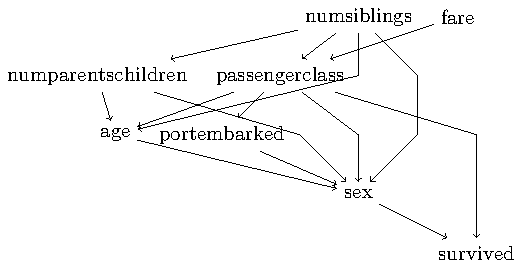
\includegraphics[width=0.5\textwidth]{../output/small/small.pdf}
    \caption{Small Dataset Graph}
\end{figure}

\begin{figure}[h]
    \centering
    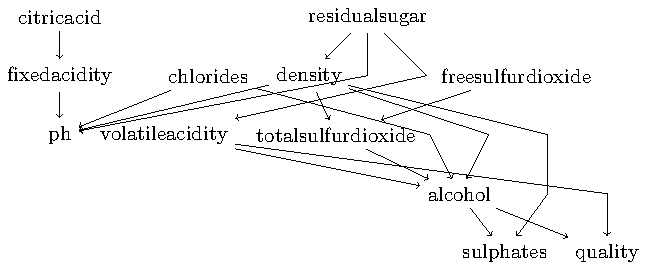
\includegraphics[width=0.5\textwidth]{../output/medium/medium.pdf}
    \caption{Medium Dataset Graph}
\end{figure}

\begin{figure}[h]
    \centering
    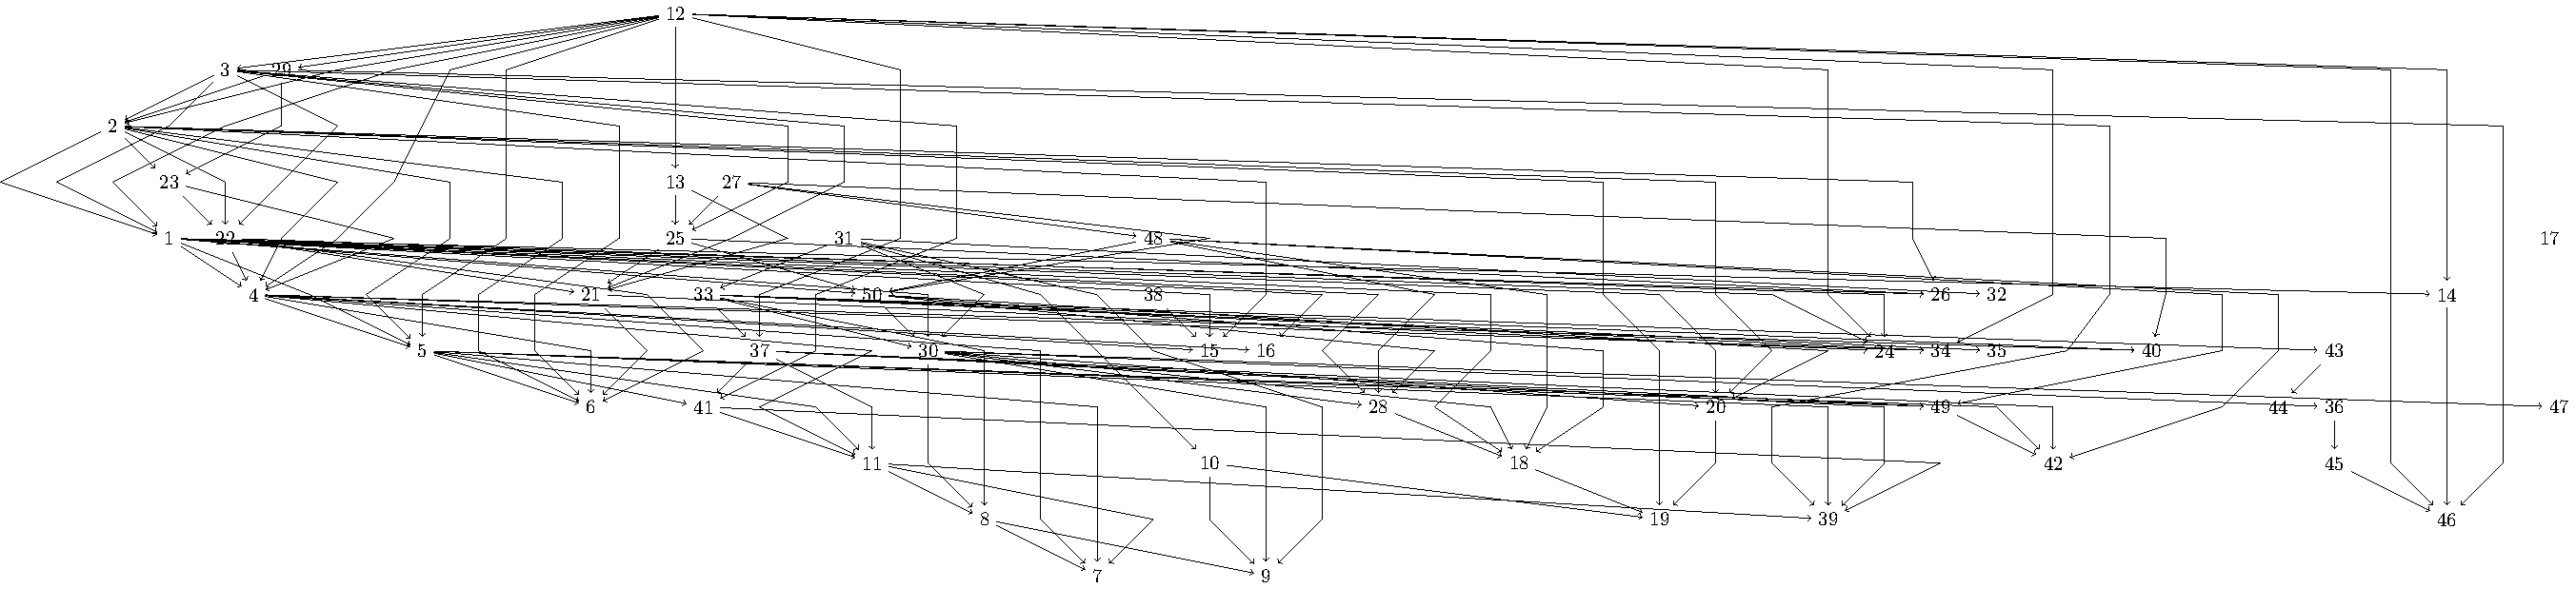
\includegraphics[width=\textwidth]{../output/large/large.pdf}
    \caption{Large Dataset Graph}
\end{figure}

\section{conclusion}
A more thorough treatment of this algorithmic approach would have likely yielded better results. This includes tuning the weighting parameters for updating particle positions, adding consideration of the best solution in the neighborhood of each particle, and varying the number of particles per simulation.

\section{Code}
\begin{algorithm}
\begin{lstlisting}[language=Julia]
########################################################################
#                           JULIA PACKAGES                             #
########################################################################
using LinearAlgebra
using LightGraphs
using DataFrames
using CSV
using Printf
using SpecialFunctions
using TikzGraphs
using TikzPictures
using Random

########################################################################
#                              USER STRUCTS                            #
########################################################################
struct Variable
    name::Symbol
    m::Int
end

mutable struct Particle
    i::Int                  # particle number
    pos::Vector{Int}        # current particle position
    vel::Vector{Float64}    # current particle velocity
    score::Float64          # current particle score
    pos_pbest::Vector{Int}  # best    particle position
    score_pbest::Float64    # best    particle score
    """
        Constructor Particle(i::Int, n_vars::Int)

    Initialize particle with bounded random position and velocity and
    -Inf score
    """
    function Particle(i::Int, n_vars::Int)
        zn = zeros(n_vars)
        pos_0 = shuffle([1:n_vars...])
        return new(i, pos_0, rand(0:1e-5:1,n_vars), -Inf, pos_0, -Inf)
    end
end

mutable struct PSO
    P::Vector{Particle}     # array of n_p particles
    n_p::Int                # number of particles used in process
    n_vars::Int             # number of variables in graph
    pos_gbest::Vector{Int}  # global best particle position
    score_gbest::Float64    # global best particle score
    mut_frac::Float64       # percentage of particles to mutate at each iteration
    mut_n::Int              # number of mutations (2 * number of swaps)
    search_fcn              # function handle of graph search function
    gbest_i::Int            # number of iterations with same gbest score
    gbest_i_max::Int        # termination condition
    """
        Constructor PSO(n_p::Int, n_vars::Int, search_fcn)

    Initialize particle swarm optimization process with i particles,
    n_vars graph variables, and search algorithm search_fcn. Set initial
    gbest position to zeros and gbest score to -Inf. Set default 
    parameters as: mut_frac=0.1, mut_n=2, gbest_i_max=5.
    """
    function PSO(n_p::Int, n_vars::Int, search_fcn)
        P = [Particle(i, n_vars) for i in 1:n_p]
        return new(P, n_p, n_vars, zeros(Int, n_vars), -Inf, 0.1, 2, search_fcn, 0, 5)
    end
end

########################################################################
#                         OUTPUT FUNCTIONS                             #
########################################################################
"""
    write_gph(dag::SimpleDiGraph, idx2names, filename)

Takes a SimpleDiGraph, a Dict of index to names and a output filename to write
the graph in `gph` format.
"""
function write_gph(dag::SimpleDiGraph, idx2names, filename)
    open(filename, "w") do io
        for edge in edges(dag)
            @printf(io, "%s,%s\n", idx2names[src(edge)], idx2names[dst(edge)])
        end
    end
end

"""
    write_score(score::Float64, filename::String)

Write score to <filename>.score.
"""
function write_score(score, filename)
    open(filename, "w") do io
        @printf(io, "%f", score)
    end
end

"""
    write_image(dag::SimpleDiGraph, filename::String)

Create visualization directed acyclical graph dag and save to 
<filename>.pdf.
"""
function write_image(dag::SimpleDiGraph, filename)
    t = TikzGraphs.plot(dag)
    TikzPictures.save(PDF(filename),t)
end

"""
    output(
        graph_struct::SimpleDiGraph,
        best_score::Float64,
        var_names::Array{String},
        file_output::String
    )

Wrapper for outputting .gph, .score, and .pdf files.
"""
function output(
    graph_struct::SimpleDiGraph,
    best_score::Float64,
    var_names::Array{String},
    file_output::String
)

    file_output_graph = file_output*".gph"
    file_output_fig = file_output
    file_output_score = file_output*".score"

    write_gph(graph_struct, var_names, file_output_graph)
    write_image(graph_struct, file_output_fig)
    write_score(best_score, file_output_score)
end

########################################################################
#                          BAYES NET FUNCTIONS                         #
########################################################################

"""
    get_n_var_values(
        graph_vars::Vector{Variable}, 
        graph_struct::SimpleDiGraph,
        n_vars::Int
    )

Get the number of possible values (r_i) for each variable in graph_vars.
"""
function get_n_var_values(
    graph_vars::Vector{Variable}, 
    graph_struct::SimpleDiGraph,
    n_vars::Int
)
    # Number of possible values (instantiations) for each variable.
    n_var_values = [graph_vars[i].m for i in 1:n_vars]

    return n_var_values
end

"""
    get_n_pa_values(
        graph_vars::Vector{Variable}, 
        graph_struct::SimpleDiGraph,
        n_vars::Int,
        n_var_values
    )

Get the number of possible parental instantiations (q_i) at each node for
each possible node value (k).
"""
function get_n_pa_values(
    graph_vars::Vector{Variable}, 
    graph_struct::SimpleDiGraph,
    n_vars::Int,
    n_var_values
)
    # Number of possible values (instantiations) for the parents of each variable.
    n_pa_values = [prod([n_var_values[j] for j in inneighbors(graph_struct, i)]) for i in 1:n_vars]

    return n_pa_values
end

function sub2ind(siz, x)
    k = vcat(1, cumprod(siz[1:end-1]))
    return dot(k, x .-1) + 1
end

"""
    bayes_net_counts(
        graph_vars::Vector{Variable}, 
        graph_struct::SimpleDiGraph, 
        dataset::Matrix{Int}, 
        n_vars::Int
    )

Given a set of variables, a graph structure, and discrete data set, 
compute the count matrices for each variable.
"""
function bayes_net_counts(
    graph_vars::Vector{Variable}, 
    graph_struct::SimpleDiGraph, 
    dataset::Matrix{Int}, 
    n_vars::Int
)
    # Number of possible values (instantiations) for variable and their parents
    n_var_values = get_n_var_values(graph_vars, graph_struct, n_vars)
    n_pa_values = get_n_pa_values(graph_vars, graph_struct, n_vars, n_var_values)

    # Pre-allocated matrix to store counts for variable instantiation i
    # given a parent instantiation j
    count_matrix = [zeros(n_pa_values[i], n_var_values[i]) for i in 1:n_vars]

    # eachcol creates a generator that iterates over the second dimension
    # of the dataset, returning the columns as AbstractVector views
    for obs_col in eachcol(transpose(dataset))
        # first loop:
        #   loop through each observation vector in the dataset
        for i_var in 1:n_vars
            # second loop:
            #   loop through each variable in the current observation
            #   vector
            # observation value relevant to the current looping variable
            obs_value = obs_col[i_var]

            # parents of current looping variable
            parents = inneighbors(graph_struct, i_var)

            # increment the counter for the current looping variable
            # given parental instantiation j and observation value k
            j = 1
            if !isempty(parents)
                j = sub2ind(n_var_values[parents], obs_col[parents])
            end
            count_matrix[i_var][j, obs_value] += 1.0
        end
    end
    return count_matrix
end

"""
    uniform_prior(
        graph_vars::Vector{Variable}, 
        graph_struct::SimpleDiGraph, 
        n_vars::Int
    )
Returns alpha vector for uniform Dirchlet prior.
"""
function uniform_prior(
    graph_vars::Vector{Variable}, 
    graph_struct::SimpleDiGraph, 
    n_vars::Int
)
    # Number of possible values (instantiations) for variable and their parents
    n_var_values = get_n_var_values(graph_vars, graph_struct, n_vars)
    n_pa_values = get_n_pa_values(graph_vars, graph_struct, n_vars, n_var_values)
    return [ones(n_pa_values[i], n_var_values[i]) for i in 1:n_vars]
end

"""
    bayesian_score_component(
        count_matrix::Vector{Matrix{Int}}, 
        alpha::Vector{Matrix{Int}}
    )
Helper function for computing the summation in the Bayesian score equation.
"""
function bayesian_score_component(
    count_matrix,
    alpha
)
    val =  sum(loggamma.(alpha + count_matrix))
    val -= sum(loggamma.(alpha))
    val += sum(loggamma.(sum(alpha, dims=2)))
    val -= sum(loggamma.(sum(alpha, dims=2) + sum(count_matrix, dims=2)))
    return val
end

"""
    bayesian_score(
        graph_vars::Vector{Variable}, 
        graph_struct::SimpleDiGraph, 
        dataset::Matrix{Int}, 
        n_vars::Int
    )

Compute the Bayesian score associated with graph_struct according to
Algorithm 5.1 in Kochenderfer, Algorithms for Decision Making
"""
function bayesian_score(
    graph_vars::Vector{Variable}, 
    graph_struct::SimpleDiGraph, 
    dataset::Matrix{Int}, 
    n_vars::Int
)
    count_matrix = bayes_net_counts(graph_vars, graph_struct, dataset, n_vars)
    alpha = uniform_prior(graph_vars, graph_struct, n_vars)
    # alpha = [ones(size(count_matrix[i]))for i in 1:5] # should do the same thing

    # Bayesian score calculated according to P. 96, Eq. 5.5
    return sum(bayesian_score_component(count_matrix[i], alpha[i]) for i in 1:n_vars)
end

########################################################################
#                    STRUCTURE LEARNING FUNCTIONS                      #
########################################################################
"""
    function k2(
        graph_vars::Vector{Variable}, 
        graph_struct::SimpleDiGraph,
        dataset::Matrix{Int},
        n_vars::Int,
        ordering::Vector{Int}
    )

k2 algorithm for Bayesian graph structure learning. Given an ordering of
graph_vars, add edges to the graph_struct that maximize the Bayesian
score for a given dataset.
"""
function k2(
    graph_vars::Vector{Variable}, 
    graph_struct::SimpleDiGraph,
    dataset::Matrix{Int},
    n_vars::Int,
    ordering::Vector{Int}
)
    for i in 1:n_vars
        parents = []
        current_node = ordering[i]
        prev_best_score = bayesian_score(graph_vars, graph_struct, dataset, n_vars)
        while true
            best_score = -Inf
            best_parent = 0
            for j in 1:i-1
                current_parent = ordering[j]
                if !has_edge(graph_struct, current_parent, current_node)
                    add_edge!(graph_struct, current_parent, current_node)
                    current_score = bayesian_score(graph_vars, graph_struct, dataset, n_vars)
                    if current_score > best_score
                        best_score = current_score
                        best_parent = current_parent
                    end
                    rem_edge!(graph_struct, current_parent, current_node)
                end
            end
            if best_score > prev_best_score
                prev_best_score = best_score
                add_edge!(graph_struct, best_parent, current_node)
            else
                break
            end
        end

    end
    return graph_struct, bayesian_score(graph_vars, graph_struct, dataset, n_vars)
end

"""
    Method particle_eval(pso::PSO)

Evaluate the score of each particle in the pso struct using the
embedded search_fcn.
"""
function particle_eval(pso::PSO)

    # increment 
    pso.gbest_i += 1

    Threads.@threads for particle in pso.P
        _, particle.score = pso.search_fcn(particle.pos)
        if particle.score > particle.score_pbest
            particle.score_pbest = particle.score
            particle.pos_pbest = particle.pos
        end
        if particle.score_pbest > pso.score_gbest
            pso.score_gbest = particle.score_pbest
            pso.pos_gbest = particle.pos_pbest
            pso.gbest_i = 0
        end
        
    end

end

"""
    Method particle_update(pso::PSO)

Update the velocity and position of each particle.
"""
function particle_update(pso::PSO)
    for particle in pso.P
        # Compute the particle velocity update as the weighted combination
        # of current, pbest, and gbest states

        particle.vel = pso.C[1]*(particle.vel) +
                       pso.C[2]*(particle.pos_pbest - particle.pos) +
                       pso.C[3]*(pso.pos_gbest      - particle.pos) 

        # The position update produces float values. Compute the new
        # particle position by sorting by the most negative values 
        # computed in the x_i + v_i position update.
        particle.pos = particle.pos[sortperm(particle.pos + particle.vel)]
    end
end

"""
    Method particle_mutate(pso::PSO)

Mutate a mut_frac percentage of the particles by randomly swapping nodes
in the ordering list.
"""
function particle_mutate(pso::PSO)

    # compute number of particles to mutate
    n_p_mutate = Int64(ceil(pso.mut_frac*pso.n_p))

    # generate random particles to mutate
    mut_idx   = rand(1:pso.n_p, n_p_mutate, 1)

    #generate random nodes to swap
    mut_which = rand(1:pso.n_vars, n_p_mutate, pso.mut_n)

    k = 0
    for particle in pso.P[mut_idx]
        k += 1
        for j in 1:Int64(pso.mut_n/2)
            # swap each pair of random indices
            temp = particle.pos[mut_which[k,j]]
            particle.pos[mut_which[k,j]] = particle.pos[mut_which[k,j*2-1]]
            particle.pos[mut_which[k,j*2-1]] = temp
        end
    end
end

"""
    Method particle_swarm_optimization(pso::PSO)

Wrapper for running the particle swarm optimization routine. Runs until
termination condition has been met.
"""
function particle_swarm_optimization(pso::PSO)
    i = 0
    while pso.gbest_i < pso.gbest_i_max
        i += 1
        particle_eval(pso)
        particle_update(pso)
        particle_mutate(pso)
    end
end

########################################################################
#                           CODE EXECUTION                             #
########################################################################
function compute(file_dataset::String, file_output::String, n_p::Int)

    dataset_df = DataFrame(CSV.File(file_dataset))

    dataset = Matrix(dataset_df)
    var_names = names(dataset_df)

    n_vars = size(dataset,2)
    graph_struct = SimpleDiGraph(n_vars)
    graph_vars = [Variable(Symbol(var_names[i]),findmax(dataset[:,i])[1]) for i in 1:n_vars]

    for i in 1:n_vars
        @printf("Variable: %s, # Values: %i\n", graph_vars[i].name, graph_vars[i].m)
    end

    search_fcn(ordering::Vector{Int}) = k2(graph_vars, SimpleDiGraph(n_vars), dataset, n_vars, ordering)
    pso = PSO(n_p, n_vars, search_fcn)

    particle_swarm_optimization(pso)

    graph_struct, best_score = pso.search_fcn(pso.pos_gbest)

    @printf("\tFinal Results: \n\t Score: %f \n\t Ordering: ", pso.score_gbest)
    for i in 1:pso.n_vars
        @printf("% i", pso.pos_gbest[i])
    end

    output(graph_struct, best_score, var_names, file_output)

end

runcases = ["small","medium","large"]
which_run = [2]

for i in which_run
    file_dataset = joinpath(@__DIR__,"..","data",runcases[i]*".csv")
    file_output = joinpath(@__DIR__,"..","output",runcases[i],runcases[i])

    @time compute(file_dataset, file_output, 4)
end
\end{lstlisting}
\end{algorithm}
\begin{thebibliography}{3}
\bibitem{paper1}
Cooper, G. F., \& Herskovits, E. (1992). A Bayesian Method for the Induction of Probabilistic Networks from Data. Machine Learning, 9(4), 309–347. https://doi.org/10.1023/A:1022649401552
\bibitem{paper2}
Ruiz, C. (2005). Illustration of the K2 algorithm for learning Bayes net structures. WPI Department of Computer Science, 1–7. http://web.cs.wpi.edu/~cs539/s07/Projects/k2\_algorithm.pdf
\bibitem{paper3}
Aouay, S., Jamoussi, S., \& Ayed, Y. Ben. (2013). Particle swarm optimization based method for Bayesian Network structure learning. 2013 5th International Conference on Modeling, Simulation and Applied Optimization, ICMSAO 2013, 0–5. https://doi.org/10.1109/ICMSAO.2013.6552569
\end{thebibliography}
\end{document}
